%%%%%%%%%%%%%%%%%%%%%%%%%%%%%%%%%%%%%%%%%%%%%%%%%%%%%%%%%%%%%%%%%%%%%%%%%%%%%%%%
%                                                                              %
%   File:     metholodgy.tex                                                   %
%   Document: XXX	                                                           %
%   Author:   Freismuth David                                                  %
%	Date:	  22.JUN.2018                                                      %
%   Content:  Contains the Metholodgy section of the Bachelor thesis.          %
%                                                                              %
%%%%%%%%%%%%%%%%%%%%%%%%%%%%%%%%%%%%%%%%%%%%%%%%%%%%%%%%%%%%%%%%%%%%%%%%%%%%%%%%

%%%%%%%%%%%%%%%%%%%%%%%%%%%%%%%%%%%%%%%%%%%%%%%%%%%%%%%%%%%%%%%%%%%%%%%%%%%%%%%%
\section{Metholodgy}

To achieve our goal of the categorization of hardware designs trough a structural analysis of the corresponding HDL Design, we firstly propose a non-standardized match vector, which contains the count of the Design's Two-to-One and One-to-One Gate Level Connections (see \label{logicGates} referencce) as each of its entries, and secondly a standardized match vector, which reduces the information hold by the non-standardized match vector down to a two dimensional vector. This standardized match vector shall then act as categorization criteria, to sort the design into predefined design categories. Those categories are clusters in the vector space the standardized match vector is part of. If the match vector points into such a cluster, the design is identified with the corresponding category.
This section elaborates on the details of finding a match vector of a design, and
how the category clusters are defined. 

\subsection{Cluster Identification}
As mentionend above, before any categorization can take place, the categories itself
have to be defined. In our model, categories are clusters in a two dimensional vector space. 
Therefore, the task is to identify clusters in this vector space, and name them. 
To do this, we determine the match vectors of well known designs. Since
the categorization of those designs is already available, the vectors that originate from designs with identical categorizations, can be grouped together to clusters. 

It is expected, that the validity of such clusters increases with the number of analyzed designs. Therefore an automatic process has to be established, to enable the analysis of a great amount of designs. To achieve this, Scrapy, a Python web scraping tool, is used to automatically obtain design files and corresponding meta-information. \gls{oc} serves as source for those design files. Among the set of information that is specifically provided for each design by \gls{oc}, we fetch and process following information.  

\begin{enumerate}

	\item{\gls{url} to the design archive}
        So the Cluster Identification can be validated at a later point in time (asuming the files still exist under the same link).

	\item{The name of the design project}
        Used to address single designs. 

	\item{The \gls{hdl} in which the design is specified and implemented}
        Necesarry for the synthesis process, later in the cluster identification process

	\item{The category in which a design is listed}
        Mandatory for the Cluster identification process. 
        
	\item{The \gls{hdl} files of the design}
        Trivially necesarry.
        
\end{enumerate}

Scrapy is able to process data with a pipeline structure, which, in our case, enables us to push user defined data sets trough those stages, an perform specific actions on them. The advantage herein lies in the parallelity that can be achieved by using this strucutre, since multiple pipelines can be active at a given time. \cref{fig:scrapyPipeline} shows the pipeline stages of the scrapy implementation in this context.
The following chapters explain in detail, how those Pipeline stages manipulate the data stated in the enumeration above.

\begin{figure}
    \centering
    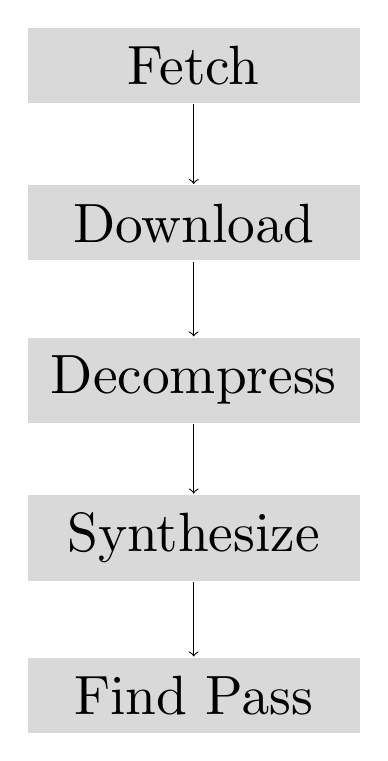
\begin{tikzpicture}[scale = 2]
        \tikzstyle{every node} = [scale = 2, rectangle, fill=gray!30, minimum width = 6em, minimum height = 1em)]
        \node(Fetch) at (0,0) {Fetch};
        \node(Download) at (0,-1) {Download};
        \node(Decompress) at (0,-2) {Decompress};
        \node(Synthesize) at (0,-3) {Synthesize};
        \node(Find pass) at (0,-4) {Find Pass};
        \draw [->] (Fetch) -- (Download);
        \draw [->] (Download) -- (Decompress);
        \draw [->] (Decompress) -- (Synthesize);
        \draw [->] (Synthesize) -- (Find pass);

    \end{tikzpicture}
    \label{fig:scrapyPipeline}   
    \caption{ Pipeline stages of the \gls{scrapy} implementaion. As seen in the figure, Pipelines can be executed parallelily. Although the final Stage "Clustering" waits on all pipelines to finish. }
\end{figure}

\subsubsection{Fetch} 
\gls{oc} does not offer an interface to automatically download all available design files. Therefore it has to be resorted to the web page, which is optimized for human interaction, but not for machine readability. Tools, which are spezialized in translating human readable content into structured, machine oriented data sets, are called \glspl{scraper}. \gls{scrapy} is one of them, and provides multiple python classes which enable extensible web scraping.

Scrapy's input is the HTML representation of the web page, which it is able to retrieve by itself, by providing a URL link to the web page. The HTML code is scanned for its elements.  Those are then parsed into python classes, and exposed to the user. The content of the parsed classes can be reorganized into user defined python classes, and passed to other user defined functions, which, among others, can store those informations persistently on a filesystem. Another option is to use HTML objects like Hyperlinks to further fork into the web page.

\begin{lstlisting}[style = python, caption = {Scrapy Main Class}]
 class IPspider_oc(scrapy.Spider):
    """The class, which is called by the scrapy framework. """
    name = 'ipspider_oc'   # the name of the spider

    def start_requests(self):
        return [scrapy.Request(
          url = "https://opencores.org",
          callback=self.login)]

    def login(self, response):
        return scrapy.FormRequest.from_response( 
          response, 
          formdata={'user' : 'davFreismuth',  
                    'pass' : 'Qlghkeul'}, 
          callback=self.redirect )

    def redirect(self,  response):
        return scrapy.Request( 
          url = "https://opencores.org/projects?lang=0&stage=5&license=0&wishbone_version=0", 
          callback=self.parse )
                                                
    def parse(self, response):
        """Default callback for scrapy. Starts at start_url, fetches the url of the different project pages, and calls parse_metadata for each project page"""
        for href in response.css('td.project a::attr(href)'):
            yield response.follow(href, self.parse_metadata)

    def parse_metadata(self, response):
        """parses metadata of an opencore.org project page and returns a scrapy item object."""
        def scrape_line(strArray,  removeStr):  
            '''helper function which iterates trough the string array 'strArray', selects the first entry which contains 'removeStr' and returns the string without removeStr and whitespaces.'''
            for str in strArray:
                if(str.find(removeStr) != -1):
                    retStr = str.replace(removeStr,  '')
                    return retStr.strip()
            
        def scrape_href(line):  
            """helper function, which gets an html <a> element, checks if it has inner html and returns the text of the inner html"""
            start = line.find(">")
            end = line.find("<", start)
            if((start + 1) == end):
                return ""
            else:
                return line[(start+1):(end)]
            
        #fill up the fields
        hdl_IP =  HDL_IP()
        hdl_IP['name'] = scrape_line(response.css('h2 + p::text').extract(), 'Name:')
        hdl_IP['created'] = scrape_line(response.css('h2 + p::text').extract(), 'Created:')
        hdl_IP['updated'] = scrape_line(response.css('h2 + p::text').extract(), 'Updated:')
        hdl_IP['file_urls'] = ['https://opencores.org' + response.css('p a::attr(href)')[1].extract()]
        category = scrape_href(response.css('p a')[5].extract())
        category = category.lower()
        category = category.replace(' ', '_')
        hdl_IP['category'] = category
        hdl_IP['language'] = scrape_href(response.css('p a')[6].extract())
        hdl_IP['license'] = scrape_line(response.css('h2 + p::text').extract(),  'License:')
        hdl_IP['basePath'] = self.settings['FILES_STORE']
        yield hdl_IP
\end{lstlisting}


\paragraph*{Authentication \\}

For our application, the first challenge is, to authenticate via the \gls{oc} user system, since designs are only downloadable while logged in with a cost free \gls{oc} account. Login information is often communicated via HTML POST Messages, which encode the message content into the message header. In the login case, the login information is encoded into the header. The web page returns an authentication token, which is stored as cookie and enables access to the web page. Scrapy is natively able to generate send such POST messages and exposes the answer to such a POST messages in Python classes, for further actions. 




\paragraph*{Traversing of the Web Page \\}

As \gls{oc}'s web page is built, like most web pages, in a tree like structure (see <<LABEL>> for reference), scrapy has been configured to start from the root page <<URL>>, where the links to all projects reside. It then calls each project page, by filtering for the <h> elements of the 

Like most web pages, \gls{oc} is built in a tree-like structure.  
The scraped data is temporarily stored into Python class objects. The information 
in these objects are written to a .JSON file, in order to make them persistent (such
that we do not have to scrape the entire \gls{oc} web site every time we use our 
classification framework). For this .JSON file, a specific format has been defined, 
so information can be imported from other sources then scrapy aswell. 

\begin{figure}[h]
	\centering
	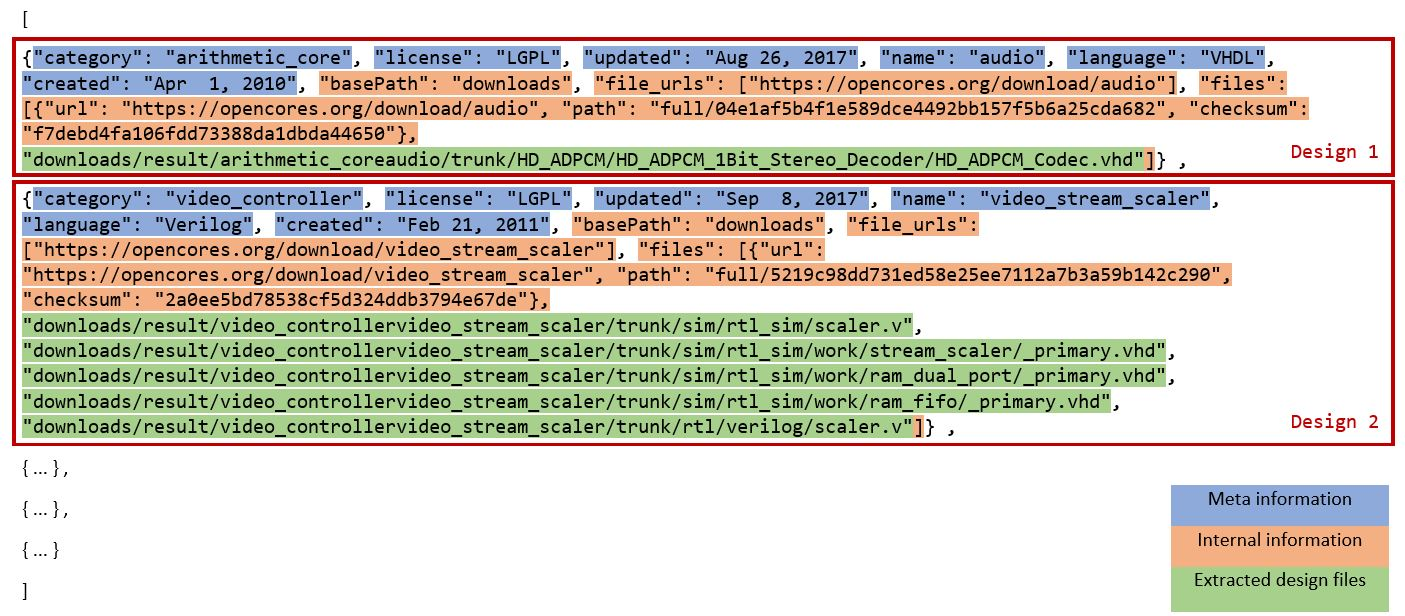
\includegraphics[width=\textwidth,keepaspectratio]{fig/jsonFileFormatDescription.JPG}
	\caption{.JSON File Format Description}
	\label{fig:jsonFormat}
\end{figure}

Figure \Cref{fig:jsonFormat} shows an example of the content of the .JSON file. 

\subsubsection{Downloading OpenCores projects}
The Scrapy python module provides the functionallity to automatically download and
store files that are associated with a Hardware design project, to a predefined
folder. Since \gls{oc} requires an account to be able to download hardware designs, 
we use a scrapy internal function to send a POST request to the \gls{oc} webpage,
in order to authorize ourselfs. 

Because all project files from the \gls{oc} database are provided as tar.gz archives,
we introduced an additional decompression step.  

\subsubsection{Decompressing design files} 
Projects from \gls{oc} are solely provided as *.tar.gz compressed archive. The \gls{python}
module tarfile enables the extraction of those archives. Additionally 
to the decompression, we sort the project files into folders corresponding to 
their associated hardware category (as stated by \gls{oc}). After that, the file 
endings of the files are analysed. If those endings indicate a \gls{hdl} file, the path 
to this file is added to the aforementioned .JSON file, in order to be able to
address the design files of a project in later steps.

\subsubsection{Reading designs into synthesis tool} 
After the design has been decompressed, it is time to let the synthesis tool 
yosys read the design files and synthesise them into a text file format. In 
order to do this, yosys expects a yosys script file, which holds all yosys commands 
that should be executed on a set of files. This script file can either be provided
by the user before a programm run, or a generic one can be generated automatically 
during a programm run, according to the files that have been provided with the 
.JSON file. 

The synthesis tool's frontend is chosen based on the language of each design file.
For \gls{vhdl} and SystemVerilog, the \lstinline{verific} frontend is used. For Verilog,
we use the \lstinline{read_verilog} frontend. Once any combination of \gls{hdl} files
has been loaded, a synthesize run attempts to generate a single HDL file from the provided
files, which solely contains primitive logic blocks. 

Since yosys does not support automatic dependency recognition of vhdl files, a custom solution
had to be found, to determine the load order of vhdl files (in the case that the user decides
that yosys scripts should be generated automatically). To accomplish this, we slightly modified 
the Vunit python project, which offers a function to return the \gls{vhdl} 
files in an ordered list. The vhdl files can then be loaded in the order dictated by this list.  

\subsubsection{Naming designs} 
Each design that is read by the synthesis tool is named after the project from
which the design files are downloaded. From then, the design name is the main
reference for each design and serves as identification feature in all
subsequent steps.

\subsubsection{Matching designs against standard pattern vector}
\subsubsection{Calculating clusters of design match vectors}

\subsection{Design Identification}
blabla

\subsection{Verification}
blabla



